%iffalse
\let\negmedspace\undefined
\let\negthickspace\undefined
\documentclass[journal,12pt,onecolumn]{IEEEtran}
\usepackage{cite}
\usepackage{amsmath,amssymb,amsfonts,amsthm}
\usepackage{algorithmic}
\usepackage{graphicx}
\usepackage{textcomp}
\usepackage{xcolor}
\usepackage{txfonts}
\usepackage{listings}
\usepackage{enumitem}
\usepackage{mathtools}
\usepackage{gensymb}
\usepackage{comment}
\usepackage[breaklinks=true]{hyperref}
\usepackage{tkz-euclide} 
\usepackage{listings}
\usepackage{gvv}                                        
%\def\inputGnumericTable{}                                 
\usepackage[latin1]{inputenc}                                
\usepackage{color}                                            
\usepackage{array}                                            
\usepackage{longtable}                                       
\usepackage{calc}                                             
\usepackage{multirow}                                         
\usepackage{hhline}                                           
\usepackage{ifthen}                                           
\usepackage{lscape}
\usepackage{tabularx}
\usepackage{array}
\usepackage{float}

\usepackage{enumitem}
\usepackage{xcolor}
%\usepackage{multicol}


\newtheorem{theorem}{Theorem}[section]
\newtheorem{problem}{Problem}
\newtheorem{proposition}{Proposition}[section]
\newtheorem{lemma}{Lemma}[section]
\newtheorem{corollary}[theorem]{Corollary}
\newtheorem{example}{Example}[section]
\newtheorem{definition}[problem]{Definition}
\newcommand{\BEQA}{\begin{eqnarray}}
\newcommand{\EEQA}{\end{eqnarray}}
\newcommand{\define}{\stackrel{\triangle}{=}}
\theoremstyle{remark}
\newtheorem{rem}{Remark}

\title{1.9.12}
\author{AI24BTECH11021 - Manvik Muthyapu}
\begin{document}
\bibliographystyle{IEEEtran}

\maketitle
\bigskip

\renewcommand{\thefigure}{\theenumi}
\renewcommand{\thetable}{\theenumi}


\textbf{Question}:\\

Find the length of the segment joining $\vec{A}(-6, 7)$ and $\vec{B}(-1, -5)$. Also, find the midpoint of $\vec{AB}$.
\hfill (10, 2021)\\

\solution

\begin{table}[h!]    
  \centering
  \begin{tabular}[15pt]{ |c| c|}
    \hline
    \textbf{Variable} & \textbf{Description}\\ 
    \hline
    $\vec{A}$ & $\myvec{-6\\7}$ \\
    \hline 
    $\vec{B}$ & $\myvec{-1\\-5}$ \\
	\hline
    $\vec{M}$ & $\frac{\vec{A}+\vec{B}}{2}$\\
    \hline 
    \end{tabular}

  \label{tab 1.8.18}
\end{table}

Length of line segment is $\norm{B-A}$.

\begin{align}
	B-A &= \myvec{-1\\-5}-\myvec{-6\\7}\\
            &= \myvec{5\\-12}\\
	\norm{B-A} &= \sqrt{(B-A)^{T}(B-A)}\\
	&=\sqrt{\brak{5}^{2} + \brak{-12}^{2}} = \sqrt{169}\\
	    &= 13 
\end{align}

$\therefore$ The length of line segment is $13$ units.\\

Midpoint of line segment 
\begin{align}
	M &= \frac{A+B}{2}\\
	  &= \frac{\myvec{-6\\7} + \myvec{-1\\-5}}{2} = \frac{\myvec{-7\\2}}{2}\\
	  &= \myvec{-3.5\\1}
\end{align}

		$\therefore$ M = $\myvec{-3.5\\1}$


\begin{figure}[h!]
	\centering
	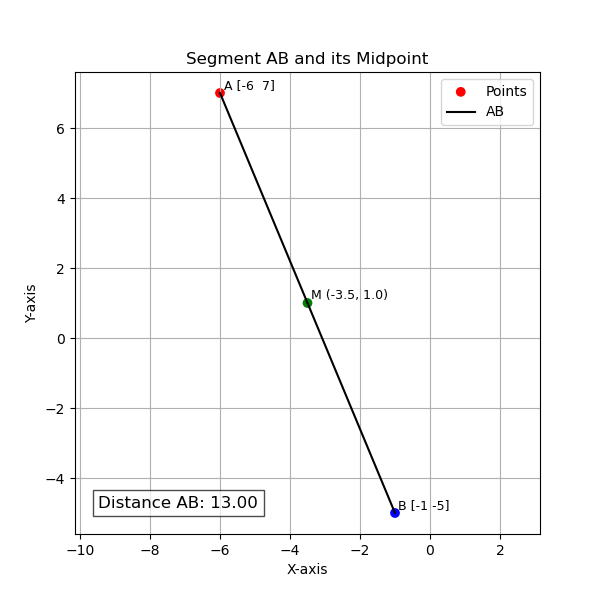
\includegraphics[width=0.7\linewidth]{figs/plot.png}
\end{figure}
\end{document}
